\subsection{Smoking Habits Among Mothers}
The mothers' smoking habit during pregnancy can have a range of negative effects on both the mother and the developing fetus. Some of the potential effects of smoking during pregnancy include:

\begin{enumerate}
    \item Increased risk of miscarriage: Smoking during pregnancy increases the risk of miscarriage, especially during the first trimester.
    \item Preterm delivery: Smoking during pregnancy can increase the risk of delivering the baby before 37 weeks of gestation, which can lead to a range of health problems for the baby.
    \item Low birth weight: Babies born to mothers who smoke during pregnancy are more likely to have a low birth weight, which can lead to a range of health problems, including developmental delays, infections, and breathing difficulties.
    \item Sudden infant death syndrome (SIDS): Babies born to mothers who smoke during pregnancy are at a higher risk of SIDS, which is the sudden and unexplained death of an otherwise healthy baby.
    \item Respiratory problems: Smoking during pregnancy can cause respiratory problems for the developing fetus, including asthma and other lung diseases.
    \item Behavioral problems: Children born to mothers who smoke during pregnancy may be more likely to experience behavioral problems, such as ADHD and conduct disorder.
\end{enumerate}

It's important for mothers to quit smoking during pregnancy to protect the health of their developing fetus and their own health as well. If you're a smoker and pregnant, you should talk to your doctor about strategies for quitting smoking and improving the health of your baby.

In overall Australia, we can see \textbf{(figure \ref{fig:smoking_au})} that mothers who smoked has increased in number.
\begin{figure}
  \centering
  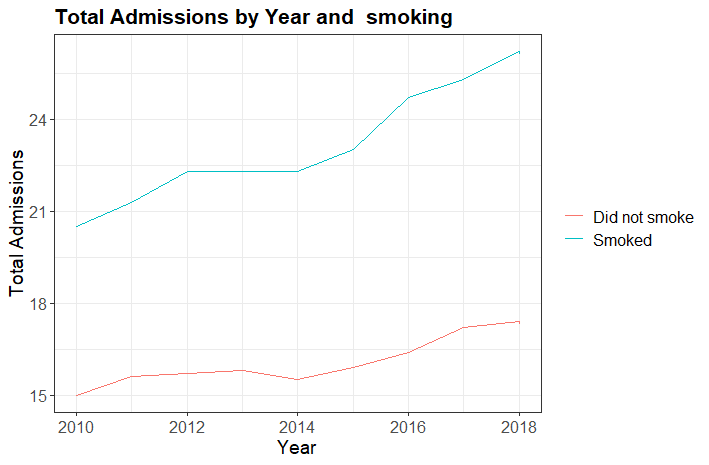
\includegraphics[width=.75\textwidth]{subsections/smoking/smoking_aus.png}
  \caption{Mother's smoking habit in ACT}
  \label{fig:smoking_au}
\end{figure}

Oppositely \textbf{figure \ref{fig:smoking_prop}} we can see that smoking was quite common among mothers of ACT in 2001 but the rate steadily decreased and came down to less than 5\% in recent years.

\begin{figure}
  \centering
  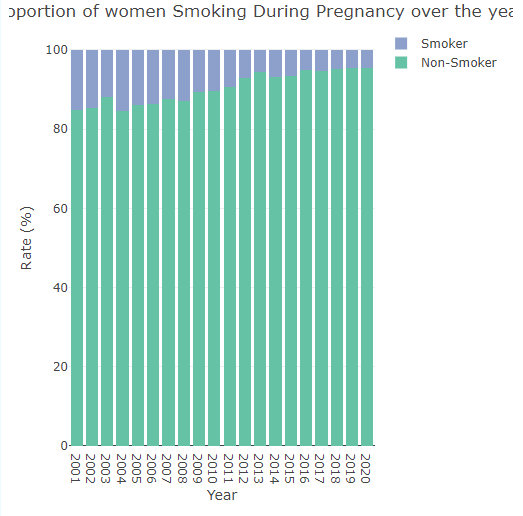
\includegraphics[width=.75\textwidth]{subsections/smoking/smoking_proportion.png}
  \caption{Mother's smoking habit in ACT}
  \label{fig:smoking_prop}
\end{figure}

\subsubsection{Mortality vs Smoking}
As we have discussed previously, smoking is directly related to mortality rate, we came up with an analysis that visualizes how smoking affects different categories of deaths.
We can see in \textbf{Figure \ref{fig:smoking-mortality}} that neonatal death is the highest among mothers who smoked during pregnancy.

\begin{figure}
  \centering
  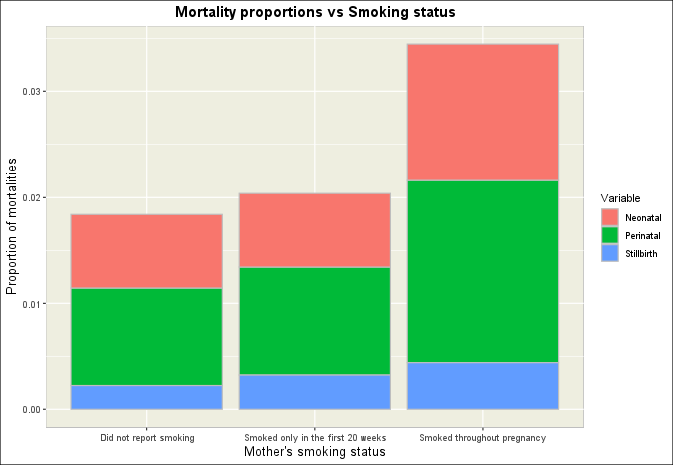
\includegraphics[width=1\textwidth]{subsections/smoking/mortality_vs_smoking.png}
  \caption{neonatal}
  \label{fig:smoking-mortality}
\end{figure}
\subsubsection{Smoker's Age in ACT}
We wanted to find out the correlation between mothers who smoke and their age among the mothers who live in ACT (\textbf{figure \ref{fig:smoking_age}}). We can see that smoking is more common among young mothers. Mothers aged 15-19 are significant in number when it comes to smoking habits. The rate falls drastically as the age increases.
\begin{figure}
  \centering
  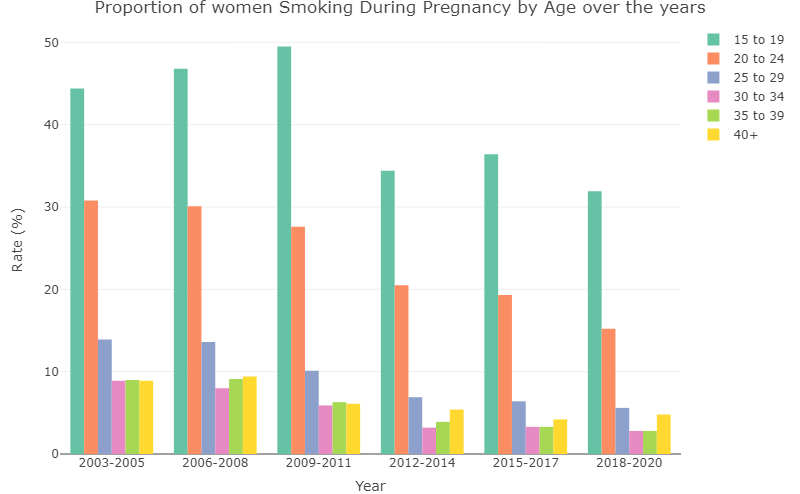
\includegraphics[width=1\textwidth]{subsections/smoking/smoking.png}
  \caption{Age groups of smoking mothers}
  \label{fig:smoking_age}
\end{figure}